\section{本章の概要}
本章では,本システムの概要について述べる.
本システムは,eラーニングで学習している学習者を対象としたシステムで,コンセプトマップを利用して学習者が学習目標を設定する場合に本システムを利用することを想定している.
本システムを利用して学習を進めることで,コンセプトマップにより自身の学習分野に対する構造的な理解を促進できるだけでなく,自身が進めている学習分野の主観的な知識獲得量を客観的に把握することが出来るため,学習目標を設定しやすくなる.

\ref{sec:kousei}節では,本システムの構成について述べる.
\ref{sec:env}節では,本システムの開発環境について述べる.
\ref{sec:about_system}節では,本システムにおける各機能の概要について述べる.
\ref{sec:futan}節では,本システムの運用における指導者の負担について述べる.

\section{本システムの構成}\label{sec:kousei}
本システムの構成を図\ref{fig:kousei}に示す.
本システムは,学習者がインターネットを通じて本システムのWebアプリケーションに接続することによってコンセプトマップを作成し学習を進めることができる.
本システムはすべての開発環境をDockerを用いて作成しているため,Dockerを使用できる環境であればどこでも本システムを実行することが可能である.

本システムで利用可能な学習教材は,その学習分野において教材提供者が階層構造を持つと判断した学習教材であれば利用可能である.
コンセプトマップを作成するにあたって,本システムではグラフデータベースを用いてコンセプトマップにおけるノードやリンク,リンクキーワードをグラフデータベースにおけるノード,エッジ,プロパティに変換することによってグラフデータベースにコンセプトマップのデータを保存し,その後グラフデータベースを可視化するライブラリを用いてコンセプトマップを閲覧,作成できる機能を作成した.
本システムを利用した学習手順として,学習者は指導者が作成した学習コンテンツを学び,そのフィードバックとして各問題がどのような学習分野となるのか教授してもらう.
その後,本システムを用いてそれぞれの学習分野をコンセプトマップを用いてどのような階層構造になっているのかを予測しながらコンセプトマップを作成する.
最後に本システムが指導者から入力された学習分野に対する階層構造のデータからコンセプトマップを自動的に作成する.
これにより学習者は,自身が作成したコンセプトマップと,自動的に作成されたコンセプトマップとを比較することにより,学習分野における自身の階層構造に対する理解を深めることができる.
加えて本システムではコンセプトマップのノードにおいて学習者の問題の回答情報から点数によってノードの背景色を表示できる.
これにより学習者は対象学習分野について,主観的に考えていた学習理解度と実際のテストの点数による学習理解度をはっきりと視覚的に確認でき,自分は特定分野においてしっかり学修できていたと思っていたが,実際はあまり理解できてきなかったという勘違いを正すことができる.
\begin{figure}[htbp]
\begin{center}
\includegraphics[width=10cm]{img/kousei.eps}
\end{center}
\caption{システム構成}
\label{fig:kousei}
\end{figure}

\section{開発環境}\label{sec:env}
本システムは,コンテナ仮想化プラットフォームであるDockerを基盤として開発している.
指導者は,本システムの運用Webサーバが内包されたDockerイメージを自身のPC上にインポートして学習用コンテナを生成することで,Webアプリケーションを実行でき,学習者に対してコンセプトマップを用いた学習を実施できる.
また,本システムにおけるグラフデータベースであるNeo4jとPythonのWebフレームワークの一つであるFlaskを用いることによりグラフデータベースとコンセプトマップのデータ変換部をAPIを用いて作成していることにより,様々なプラットフォームで本システムのグラフデータべース+コンセプトマップという学習環境を利用する事が可能である.
以下に,本システムの利用にあたって指導者が実行しなければならないDockerコマンドを一覧に示す.

\begin{itemize}
    \item docker-compose up -d --build\\
    - 指導者のPC上に本システムのDockerイメージをインポートし実行する
    
    \item docker-compose down -v\\
    - 本システムに何か変更を加えた際にコンテナを停止させるためのコマンド

    \item docker system prune\\
    - 本システムに何か変更を加えた際にコンテナに残っているキャッシュを削除するためのコマンド
    
\end{itemize}


\section{本システムにおける各機能の概要}\label{sec:about_system}
本システムは大きく分けて3つの機能によって成り立っている.
それは,グラフデータ管理機能,グラフデータ入力補助機能,グラフデータ可視化機能の3つの機能である.
それぞれの機能について\ref{subsec:kanri}節,\ref{subsec:hojo}節,\ref{subsec:kasi}節で説明する.

\subsection{グラフデータ管理機能}\label{subsec:kanri}
グラフデータ管理機能は,学習者と指導者のグラフデータを管理する機能で,クライアントのフォームから入力されたコンセプトマップの親子に関するデータをAPIを用いてグラフデータへと変換しグラフデータベースへとデータを登録する.
また,クライアントからグラフデータを要求された場合,グラフデータをAPIを用いてJSON形式で返答する.

グラフデータ管理機能が使用するAPIは以下のとおりである.

\begin{itemize}
    \item /create/json \\
    - 与えられたJSON形式のデータをグラフデータベースで利用できるJSON形式のデータに変換し,データを登録しその結果をJSON形式で返答する.

    \item /get/all\_graphs \\
    - グラフデータベースに登録されているすべてのグラフデータをJOSN形式で返答する.

    \item /create/score \\
    - 指定されたユーザと教科の点数登録を行う.

    \item /get/score \\
    - 指定された教科に紐づくすべての点数を返答する.

    \item /get/score/\<username\> \\
    - 指定されたユーザに関する教科の得点を返答する.

    \item /get/subject/\<subject\> \\
    - 指定されたユーザが受験した科目と点数を返答する.

    \item /delete/\<string:node\_name\> \\
    - 指定されたノードを削除する.

    \item /delete/all \\
    - すべてのノードを削除する.
    
\end{itemize}

これらのAPIを利用することにより本システムはグラフデータベースとコンセプトマップを紐づけて利用している.
\newpage

\subsection{グラフデータ入力補助機能}\label{subsec:hojo}
グラフデータ入力補助機能は,クライアントでJSON形式のグラフデータを入力補助する機能である.
この機能は指導者が用いる機能で,新規にグラフデータを入力する場合に用いる.
グラフデータは,最低でも属性,親ノード,子ノードの一セットを入力する必要がある.
そのためテキストベースの従来のデータ入力フォームでは,関係性など誤って入力する可能性がある.
そこで本機能では入力フォームを階層構造で入力可能なUIとして提供し,入力誤りを減らすようにしている.
また,本入力フォームはドラック&ドロップや編集メニューを用い,入力データを階層表示し操作できる.
これにより,指導者は関係性を整理しながらグラフデータを入力することが可能である.

グラフデータ入力補助機能のGUIを図\ref{fig:hojo}に示す.

\begin{figure}[htbp]
\begin{center}
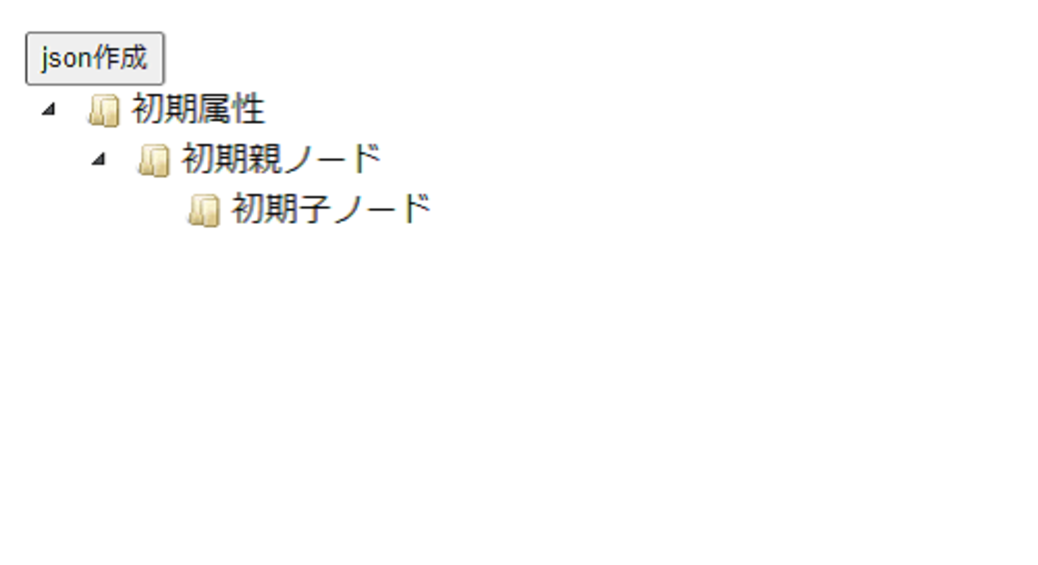
\includegraphics[width=10cm]{img/hojo.eps}
\end{center}
\caption{グラフデータ入力補助機能初期状態}
\label{fig:hojo}
\end{figure}

図\ref{fig:hojo}は初期状態で,図のような木構造な入力フォームを提示する.
初期属性とは第\ref{chap:conceptmap}章の図\ref{fig:example_concept}で示した植物に該当する.
初期親ノードは被子植物,初期子ノードはサクラに該当する.
\newpage
各々の階層は図\ref{fig:hojo_change_name}のようにして各ノードを右クリックすることによりメニューが表示される.

\begin{figure}[htbp]
\begin{center}
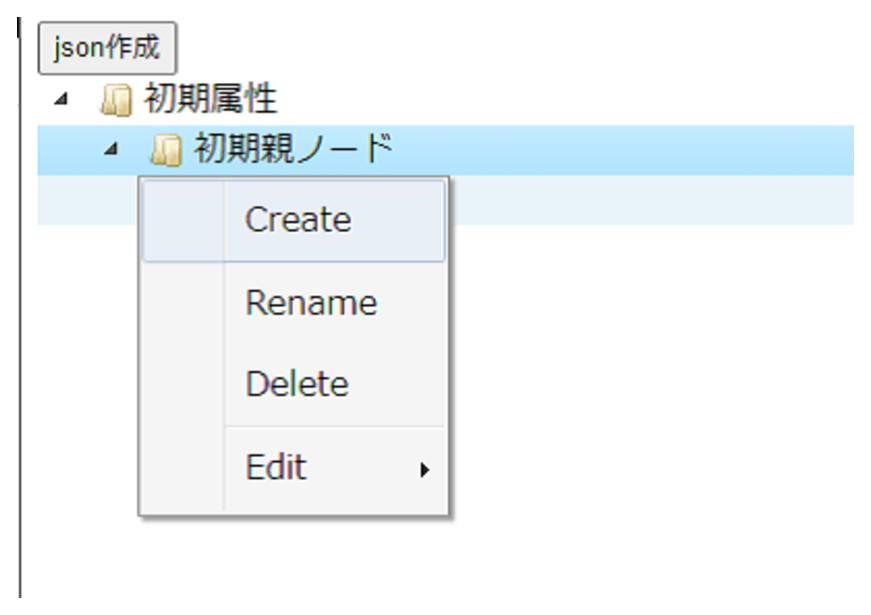
\includegraphics[width=10cm]{img/hojo_change_name.eps}
\end{center}
\caption{グラフデータ入力補助機能編集状態}
\label{fig:hojo_change_name}
\end{figure}

\newpage
メニューはCreate, Rename, Delete, Editの四種類あり,それぞれノードの新規作成,ノードの名前変更,ノードの削除,ノードの編集を意味する.
Editについては,図\ref{fig:hojo_edit}のようにして,Cut, Copy, Pasteが存在し,それぞれノードの切り取り,ノードのコピー,ノードの貼り付けが可能である.

\begin{figure}[htbp]
\begin{center}
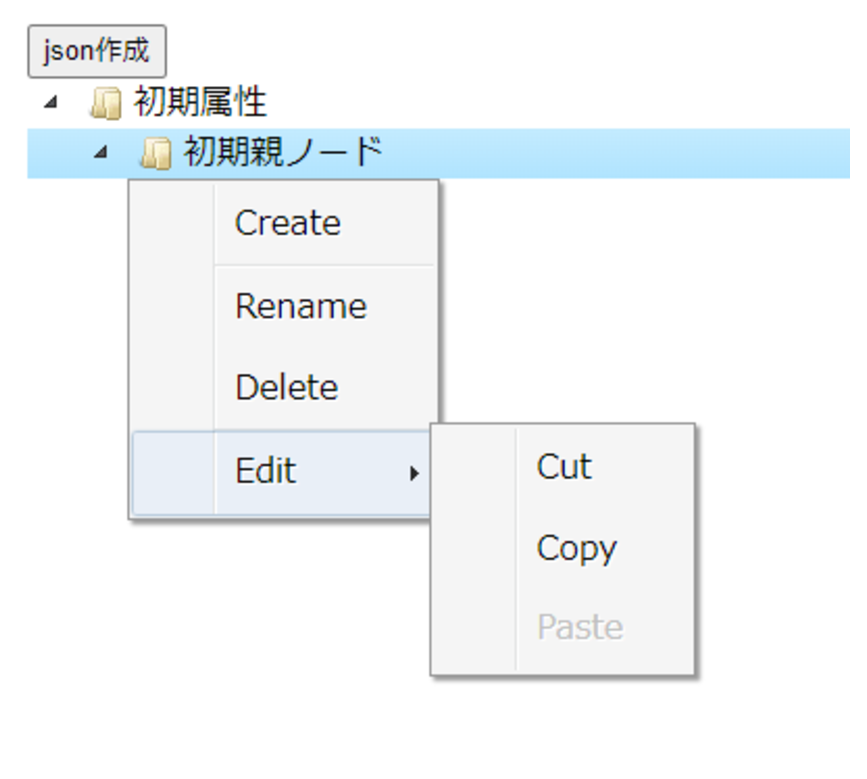
\includegraphics[width=9cm]{img/hojo_edit.eps}
\end{center}
\caption{グラフデータ入力補助機能 Editについて}
\label{fig:hojo_edit}
\end{figure}

これらの機能を指導者は用いてコンセプトマップのデータをグラフデータとしてグラフデータベースに登録できる.
\newpage
\subsection{グラフデータ可視化機能}\label{subsec:kasi}


\section{本システムの運用における指導者の負担}\label{sec:futan}
本システムの運用における負担として,グラフデータの入力作業と学習者の試験結果の得点入力作業の2つの負担要素が考えられる.
まず,グラフデータの入力作業における負担について述べる.

グラフデータの入力作業において,現在のシステムでは複数の学習分野に関するグラフデータの入力が不可能である.
しかし,一つの学習分野に絞ってグラフデータを作成する場合は本システムはグラフデータ入力補助機能により容易にグラフデータを入力できる.
このことから複数の学習分野を教える必要がある指導者にとっては本システムはやや大きい負担がかかることが考えられるが,一分野に関して指導する場合においては少ない負担になるのではと考えられる.

一方,学習者の試験結果の得点入力作業は非常に大きいと考えられる.この理由として現在のシステムでは複数の学習分野,すなわちノードに対して一括で得点を入力する機能がないことが挙げられる.
これにより指導者は学生の数x学習分野の数だけ得点データを入力しなければならず非常に負担がかかると考えられる.

上記の理由により,指導者のグラフデータ入力作業の負担はやや大きいが,学習者の試験結果の得点入力作業に関しては非常に大きな負担であると考えられる.
このため本システムでは,機能としてその負担を減らす機能は作成が不十分だったが,入力を補助するスクリプトを作成することにより今回の負担を軽減した.
今後本システムを開発するにあたってはこの負担を減らすような機能を作成できればと考えている.


